\documentclass[12pt]{report}
\usepackage{graphicx}
\usepackage{scribe_MG}
\usepackage{amssymb}
\usepackage{graphicx}
\usepackage[mathscr]{eucal}
\usepackage[english]{babel}
\usepackage[utf8]{inputenc}  %encodage du fichier
\usepackage[T1]{fontenc}
\usepackage{lmodern}
\usepackage{epstopdf}
\usepackage{array}

\usepackage{placeins}

%% William
\usepackage[colorlinks]{hyperref} % for links
\usepackage{xcolor}             % for color
\usepackage{caption}            % for caption* (without 'Figure 2.n:')
\usepackage{float}              % for H, to place figure HERE!
\usepackage{wrapfig}
\usepackage{tikz}
\usetikzlibrary{arrows}
\usetikzlibrary{positioning}

\usepackage{bbm}            % for the indicator function symbol : \mathbbm{1}
\def\R{\mathbb{R}}
\newcommand{\defobj}[1]{\color{red}#1\color{black}{}}
\newcommand{\defmean}[1]{\color{green!70!black}#1\color{black}{}}
\renewcommand{\emph}[1]{\color{violet}#1\color{black}{}}
\newcommand{\vectorline}{\rule[2px]{2em}{0.5px}}
\DeclareMathOperator{\E}{\mathbb{E}}
\DeclareMathOperator*{\argmin}{arg\,min}

\newcommand{\sigmaField}{\mathcal{E}}

% Vectors and matrices
\newcommand{\norm}[1]{\left \lVert #1 \right\rVert}
\def\XX{\mathbf{X}}
\def\wb{\mathbf{w}}
\def\xb{\mathbf{x}}
\def\yb{\mathbf{y}}
\def\ts{\top}
\def\etab{{\boldsymbol \eta}}
\def\bphi{{\boldsymbol \phi}}

% Probability and Statistics macros
\newcommand{\iid}{\overset{iid}{\sim}}
\newcommand{\normal}{\mathcal{N}}

%% For footnote horizontal spacing :
%% \usepackage{footmisc}
%% \setlength{\footnotemargin}{2mm}

\newcommand\independent{\protect\mathpalette{\protect\independenT}{\perp}}
\def\independenT#1#2{\mathrel{\rlap{$#1#2$}\mkern2mu{#1#2}}}

\newcommand{\indep}{\ensuremath{\,\bot\!\!\!\bot\,}} %% The symbol for independent
\newcommand{\notindep}{\indep\!\!\!\!\!/\,\,\,}

\newtheorem{remark}{Remark}[section]
\newtheorem{example}{Example}[section]
\newtheorem{property}{Property}[section]


\begin{document}
\coursetitle{IFT 6269: Probabilistic Graphical Models}
\semester{Fall 2016}
\lecturer{Simon Lacoste-Julien} \scribe{Zakaria Soliman}
\lecturenumber{6} \lecturedate{September 20}

\maketitle

\textbf{Disclaimer:} These notes have only been lightly proofread.

\section{Linear Regression}

\subsection{Motivation}

We want to learn a prediction function $f: \mathcal{X} \to \mathcal{Y}$. Where
$\mathcal{X} \subseteq \R^d$ and if:
\begin{enumerate}
    \item[(1)] $\mathcal{Y} = \{0,1\}$, it's a \emph{binary} classification
    \item[(2)] $\mathcal{Y} = \{0,1, \cdots, k\}$, it's a \emph{multiclass} classification
    \item[(3)] $\mathcal{Y} \subseteq \R$, it's a regression problem.
\end{enumerate}

There are several perspectives in modeling the distribution of the data:

    \subsubsection{generative perspective}
    Here, we model the joint distribution $p(x,y)$. We make more assumptions in this
    case. This leads it to be less robust for predictions (but is a more flexible approach if we are not sure what is the task we are trying to solve).
    \subsubsection{conditional perspective}
    We only model the conditional probability $p(y|x)$. Early 2000s, it was called 
    the \emph{discriminative} perspective, but Simon prefers to refer to it now as the \emph{conditional approach}.
    \subsubsection{fully discriminative perspective}
    Models $f: \mathcal{X} \to \mathcal{Y}$ directly and estimate the function $\hat{f}$ by using the loss $\ell(y,y')$ information. This approach is the most robust.


\subsection{Linear regression model}


We take a conditional approach to regression. Let $Y \in \R$ and let's assume that $Y$ depends linearly on $X \in R^d$. Linear regression
is a model of the following form:

\[
    p(y | \xb, \wb) = \normal(y | \langle \wb \,, \xb \rangle, \sigma^2)
\]

Where $\wb \in \R^d$ is the \defobj{parameter} (or \defobj{weight}) vector. Equivalently, we could also rewrite the model as

\[
    Y = \wb^{\ts} \XX + \epsilon
\]

Where the \defobj{noise} $\epsilon \sim \normal(0, \sigma^2)$ is a random variable that is independent of $X$

\begin{remark}
     Note that if there is an offset $w_0\in\R$, that is, if $Y = w_0+{\wb}^{\ts}X+\epsilon$,
     we will use an "offset" notation for $\xb$:  $$\xb = \begin{pmatrix}\tilde{\xb}\\1\end{pmatrix},$$ where
     $\tilde{\xb} \in \R^{d-1}$ and $1$ is the \defobj{constant feature}. Thus, we have:
     $$\wb^{\ts}\xb = \wb_{1:d-1}^{\ts}\tilde{\xb} + w_d$$ Where $w_d$ is the \emph{bias/offset}
 \end{remark}

 Let $D=(\xb_n,y_n)_{i=1}^n$ be a training set of conditionally i.i.d.\ random variables i.e. $X_i \sim \text{whatever}$ and $Y_i | X_i \sim \normal(\langle \wb \,, X_i \rangle, \sigma^2)$. Each $y_i$ is a \defobj{response} on
 observation $\xb_i$. We consider the \emph{conditional} likelihood of all outputs given all inputs:
 $$
 p(y_1, \cdots , y_n | \xb_1, \cdots, \xb_n ; {\wb},\sigma^2) = \prod_{i=1}^n p(y_i | \xb_i ; {\wb},\sigma^2).
 $$
 And we have that $Y_i|X_i \overset{\text{indep}}{\sim} \normal(\wb^{\ts}X_i \, , \sigma^2)$
 (i.e. $p(y_i|\xb_i) = \frac{1}{\sqrt{2\pi\sigma^2}}\exp\big( \frac{-(y_i - \wb^{\ts}\xb_i)^2}{2\sigma^2} \big)$) taking the log-likelihood gives us the following expression:
\begin{align*}
    \log p(y_{1:n}|\xb_{1:n} ; {\wb},\sigma^2) &= \sum_{i=1}^n{\log p(y_i|\xb_i)}
    \\
    &= \sum_{i=1}^n \bigg[ -\frac{(y_i - \wb^{\ts}\xb_i)^2}{2\sigma^2} - \frac{1}{2}\log(2\pi\sigma^2) \bigg]
    \\
    &= - \frac{n}{2}\log(2\pi\sigma^2) - \frac{1}{2}\sum_{i=1}^n{\frac{(y_i-{\wb}^{\ts}\xb_i)^2}{\sigma^2}}.
 \end{align*}
Notice that maximizing the likelihood comes down to the following minimization problem w.r.t. $\wb$:
$$
\begin{array}{ll}
\mathrm{find} & \hat{\wb} = \argmin_{\wb} \sum_{i=1}^n{(y_i-{\wb}^{\ts}\xb_i)^2}.
\end{array}
$$
 Define the \defobj{design matrix} $\XX$ as
 $$
 \XX = \begin{pmatrix}
 \vectorline \; \xb_1^{\ts} \vectorline
  \\ \vdots
  \\ \vectorline \; \xb_n^{\ts} \vectorline
 \end{pmatrix} \in \R^{n\times d}
 $$
 and denote by $\yb$ the vector of coordinates $\begin{pmatrix} y_1 \\ \vdots \\ y_n \end{pmatrix}$. This notation
 allows us to rewrite the residual sum of squares in a more compact fashion as:

 $$
 \sum_{i=1}^n (y_i-{\wb}^{\ts}\xb_i)^2 = \lVert \yb - \XX\wb \rVert^2
 $$
\\
 Thus, we can rewrite the log likelihood as:

 $$
 -\log p(\yb|\xb) = \frac{\lVert \yb - \XX\wb \rVert^2}{2\sigma^2} +
 \frac{n}{2}\log(2\pi\sigma^2)
 $$
\\
 Finally, the minimization problem over $\wb$ can be rewritten as:
 $$
 \begin{array}{ll}
 \mathrm{find} & \hat{\wb} = \argmin_{\wb} {\lVert \yb - \XX\wb \rVert}^2.
 \end{array}
 $$
\begin{remark}
    The minimization of ${\lVert \yb - \XX\wb \rVert}^2$ w.r.t. $\wb$ can also be
    viewed geometrically as choosing $\hat{\wb}$ so that the vector $\XX\hat{\wb}$ is the
    orthogonal projection of $\yb$ onto the column space of $\XX$
\end{remark}

Now let us find $\hat{\wb}$:

\begin{align*}
    \frac{\partial}{\partial \wb} (\yb - \XX\wb)^{\ts}(\yb - \XX\wb) &=
    \frac{\partial}{\partial \wb} \big[ \lVert \yb \rVert^2 - 2\yb^{\ts} \XX \wb + \wb^{\ts}\XX^{\ts}\XX\wb \big]
    \\
    &= 0 - 2 \XX^{\ts}\yb + 2\XX^{\ts}\XX\wb = 0 &\text{(using $\nabla_{\wb}(\wb^{\ts}\mathbf{A}\wb) = (\mathbf{A}+\mathbf{A}^{\ts})\wb)$)}
    \\
    &\iff \boxed{(\XX^{\ts}\XX)\wb = \XX^{\ts}\yb} &\text{\defobj{normal equation}}
\end{align*}

\begin{itemize}
    \item
    If $\XX^{\ts}\XX$ is invertible, there is a unique solution $\hat{\wb} = (\XX^{\ts}\XX)^{-1}\XX^{\ts}\yb$
    \item
    If $n<d$, then $\XX$ is not \emph{full rank} and so $\XX^{\ts}\XX$ is \emph{not invertible}. In this case we could use the pseudo-inverse of $\XX$, $\XX^{\dagger}$
    and choose the minimum norm $\lVert \wb \rVert$ solution amongst $\argmin_{\wb} {\lVert \yb - \XX\wb \rVert}^2$. The problem we face is that the pseudo-inverse
    is \emph{not numerically stable}.
\end{itemize}

In the latter case, it would be better to use regularization techniques (see next section).

\subsection{Ridge regression}
We can either interpret ridge regression as adding a norm regularizer to the least-square EMR, or as replacing the MLE for $\wb$ with a MAP by adding a prior $p(\wb)$:
$$\log p(\wb|\yb, \xb) = \log p(y_{1:n} | \xb_{1:n} ; \wb) + \log p(\wb) + cst$$
Where $p(\wb)$ is the prior over $\wb$ and:
$$ p(\wb) = \normal(\wb|0, \frac{\mathbf{I}}{\lambda}) $$

So we have that:
$$\log p(\wb|\yb, \xb) = \log p(y_{1:n} | \xb_{1:n} ; \wb) + cst - \frac{\lambda}{2} \norm{\wb}^2 $$
and then,
\begin{align*}
    \nabla_{\wb} = 0 &\Rightarrow (\XX^{\ts}\XX + \lambda \mathbf{I})\wb = \XX^{\ts}\yb
    \\
    &\Rightarrow \hat{\wb}_{MAP} = (\XX^{\ts}\XX + \lambda \mathbf{I})^{-1}\XX^{\ts}\yb
\end{align*}

Notice that $(\XX^{\ts}\XX + \lambda \mathbf{I})$ is always invertible.

\begin{remark}
    $-\log p(\wb|\yb, \xb)$ is \emph{strongly convex} in $\wb$. So there is a \emph{unique} global minimum
\end{remark}

\begin{remark}
    It is good practice to standardize or normalize the features. Standardizing means make the features have empirical zero mean and unit standard deviation; normalizing can mean different things, e.g. scale them to $[0,1]$ or to a unit norm.
\end{remark}

\section{Logistic Regression}
    Let's turn our attention to classification problems. For this model, we will assume that $Y \in \{0,1\}$ and $X \in \R^d$. We make no additional
    assumptions apart that $p(\xb|Y=1)$ and $p(\xb|Y=0)$ are densities. Our goal is to model $p(Y|X)$

    \begin{align*}
    p(Y=1 | X=\xb) &= \frac{p(Y=1,X=\xb)}{p(Y=1,X=\xb) + p(Y=0,X=\xb)} \\
     &= \frac{1}{1+\frac{p(Y=1,X=\xb)}{p(Y=0,X=\xb)}} \\
     &= \frac{1}{1+\exp(-f(\xb))}
    \end{align*}

    Where
    $$
       f(x) = \log \underbrace{\frac{p(X=\xb | Y=1)}{p(X=\xb | Y=0)}}_{\defobj{\text{class-conditional ratio} } } + \log \underbrace{\frac{p(Y=1)}{p(Y=0)}}_{\defobj{\text{prior odd ratio} } } 
    $$
    Is the \defobj{log odds ratio}. In general we have:
    $$p(Y=1|X=\xb) = \sigma(f(\xb))$$
    where $\sigma(z):= \frac{1}{1+e^{-z}}$ is the sigmoid function shown in Figure 2.1.

    \begin{figure}
    \begin{center}
    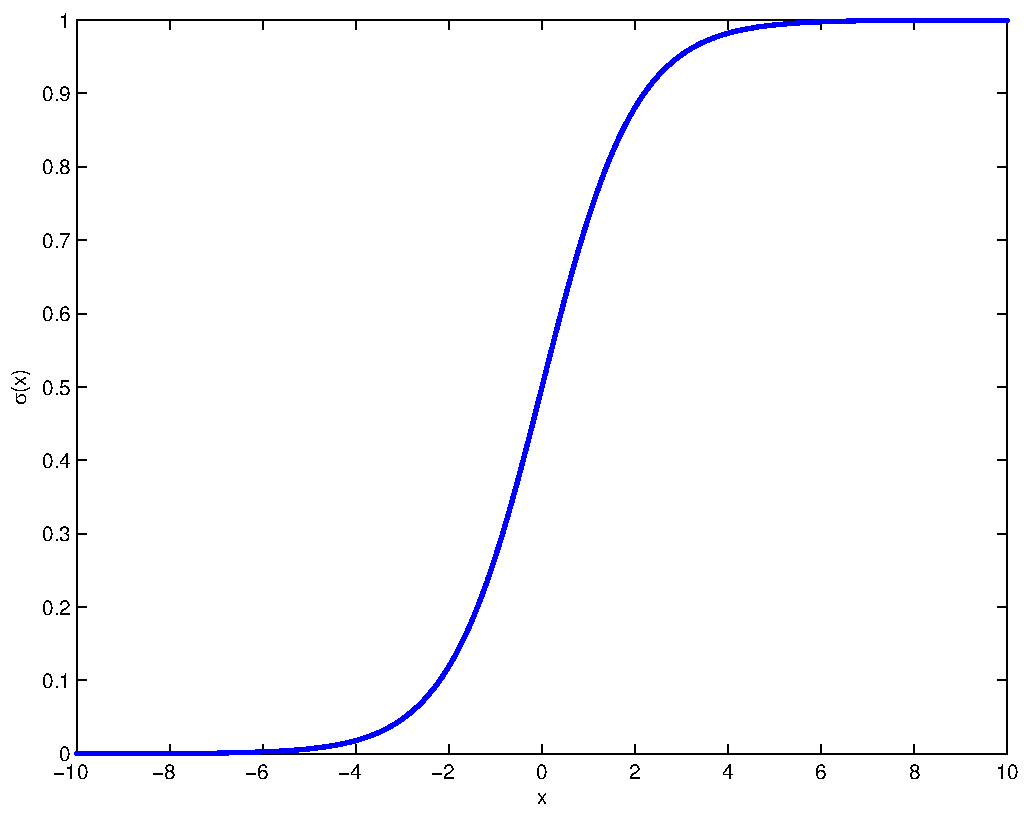
\includegraphics[width=.5\linewidth]{figures/sigmoid-eps-converted-to.pdf}
    \caption{\label{fig:sigmoid}Sigmoid function.}
    \end{center}
    \end{figure}
\pagebreak
    The sigmoid function has the following properties:

    \begin{property}
        $$
        \forall z \in \mathbb{R}, \sigma(-z)=1-\sigma(z)
        $$
    \end{property}
    \begin{property}
        $$
        \forall z \in \mathbb{R}, \sigma ' (z) = \sigma(z)(1-\sigma(z)) = \sigma(z)\sigma(-z)
         $$
    \end{property}

\begin{example}
Finally, we make the following observation that a very large class of probabilistic models yield logistic-regression types of models (thus explaining why logistic regression is fairly robust).

Consider that the class conditional is in the \emph{exponential family}:
    $$
    p(\xb|\etab) = h(\xb) \exp(\etab^\top \mathbf{T}(\xb) - A(\etab) ).
    $$

    \begin{align*}
    f(\xb) &= \log\frac{p(X=\xb | Y=1)}{p(X=\xb | Y=0)} + \log\frac{p(Y=1)}{p(Y=0)} \\
    &= (\etab_1 - \etab_0)^\top \mathbf{T}(\xb) + A(\etab_0)-A(\etab_1) + \log(\frac{\pi}{1-\pi}) \\
    &= \wb^\top \bphi(\xb)
    \end{align*}

    Where $\wb = {\etab_1-\etab_0 \choose  A(\etab_0)-A(\etab_1) + \log(\frac{\pi}{1-\pi}) }$ and $\bphi(\xb) = {\mathbf{T}(\xb) \choose  1 }$. Thus we have a logistic regression model with features $\bphi(\xb)$:

    $$
    p(y=1|\xb) = \sigma(\wb^{\ts} \bphi(\xb))
    $$

\end{example}
\end{document}
